\section{Ablation Studies}
\label{sec:ablation}
In this section, we perform ablation studies to assess the effectiveness of the methods proposed above: 
model alignment to simplify the learning task; 
inference window size to improve inference quality; 
haloing and batch-norm conditioning to increase sample quality.
\paragraph{Impact of Model Alignment.}
\begin{wraptable}{r}{0.38\linewidth}
\vspace{-8mm}
\captionof{table}{
Impact of alignment ablation and permutation on reconstruction loss.
}
\label{tab:ablation_alignment}
\small
\setlength{\tabcolsep}{6pt}
\begin{tabularx}{1.0\linewidth}{ccccc}
\toprule
\multicolumn{3}{c}{Sample Permutations} & \multicolumn{2}{c}{$\mathcal{L}_{rec}$} \\
\cmidrule(r){1-3} \cmidrule(l){4-5}
Aligned    & View 1       & View 2       & Train              & Test               \\
\cmidrule(r){1-3} \cmidrule(l){4-5}
No         & Perm.     & Perm.    & 0.304              & 0.167              \\
Yes        & Perm.     & Perm.    & 0.148              & 0.082              \\
Yes        & Align    & Perm.    & 0.107              & 0.082              \\
Yes        & Align    & Align   & 0.072              & 0.082              \\ 
\bottomrule
\end{tabularx}
\vspace{-4mm}
\end{wraptable} 
Model alignment intuitively reduces training complexity by mapping all models to the same subspace. To evaluate its impact, we conduct training experiments with the same configuration on datasets with and without aligned models. In the dataset with aligned models, we use either the aligned form or 5 random permutations for the two views for both reconstruction and contrastive learning.
As shown in Table \ref{tab:ablation_alignment}, the results show two effects. 
First, alignment through git re-basin simplifies the learning task and contributes to improved generalization, both training and test losses are reduced by more than 50\%. 
Second, anchoring at least one of the views to the aligned form does further reduce the training loss, but does not improve generalization.

\begin{wrapfigure}{r}{0.35\linewidth}
\vspace{-4mm}
\centering
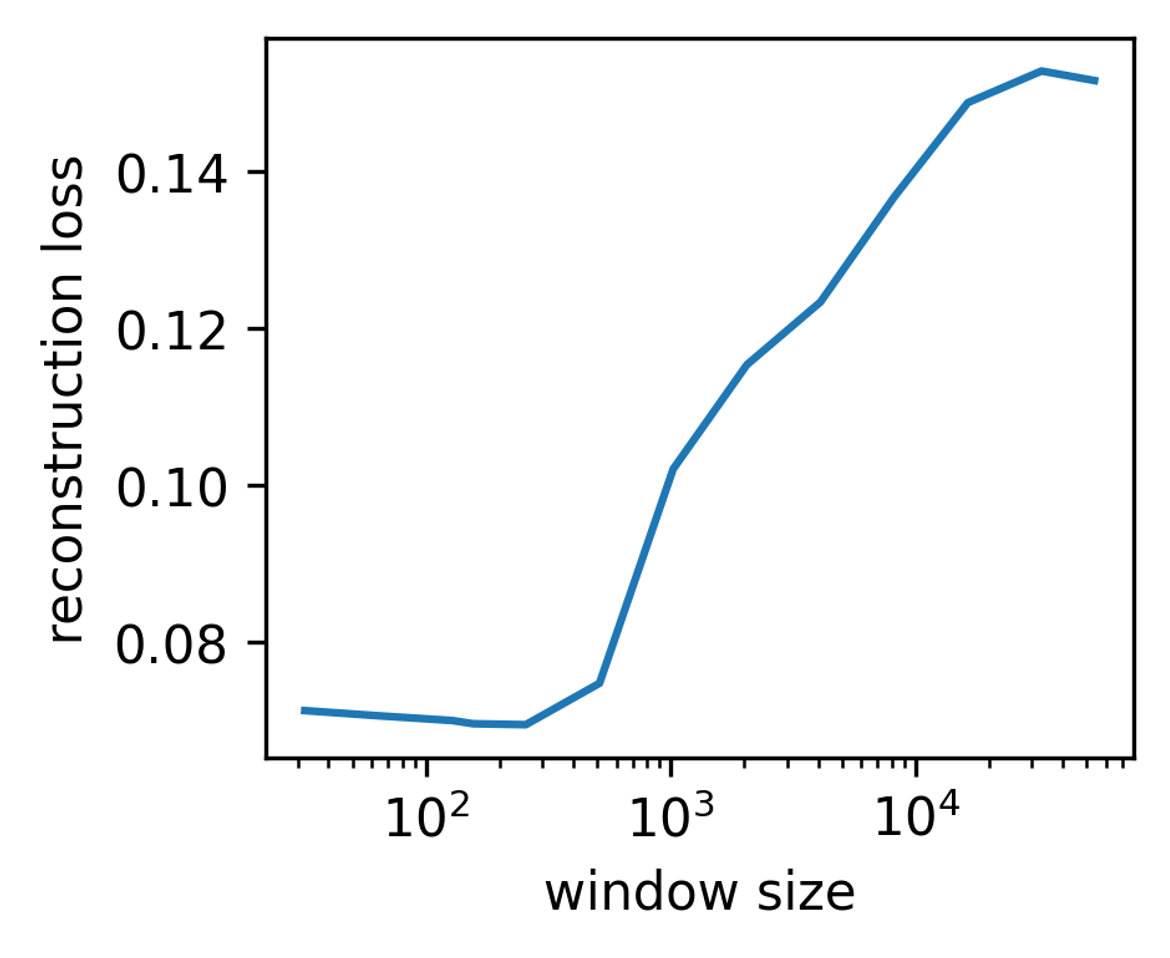
\includegraphics[trim=4mm 0mm 1.5mm 1.5mm, clip, width=1.0\linewidth]{figures/windowsize_ablation.png}
\vspace{-8mm}
\captionof{figure}{\ourmethod reconstruction loss over number of tokens within a window. The loss is lowest around the training windowsize of 256 tokens, longer sequences up to the full model sequence length of 50k tokens cause interference and double the reconstruction error.
}
\vspace{-10mm}
\label{fig:windowsize_ablation}    
\end{wrapfigure}
\paragraph{Window Size Ablation.}
The sequential decomposition of \ourmethod allows one to pretrain not on the full model sequence, but on subsequences. The choice of the length of the subsequence, the window size, is a critical parameter that balances computational load and context. We used a window of 256 for pretraining for most of our experiments. 

Here, we study the influence of the window size on reconstruction error, exploring values ranging from 32 to 2048. Our experiments did not reveal substantial impact of smaller windows on pretraining loss or sampling performance. This seems to suggest that a window size as large as 2048 may still be insufficient on ResNets to capture enough context. Alternatively, it may suggest that the underlying assumption that context matters may not entirely hold up.

However, we did observe an important impact on the relationship between training and inference window sizes. During inference, memory load is significantly lower. Inference allows much larger window sizes, up to the entire length of the ResNet sequence. However, departing from the training window size appears to introduce interference, which affects the reconstruction error (Figure \ref{fig:windowsize_ablation}). 

\paragraph{Halo and batch-norm conditioning.}
\begin{wraptable}{r}{0.35\linewidth}
\vspace{-10mm}
\captionof{table}{
Ablation of batch-norm conditioning and haloing.
}\label{tab:ablation_halo_bn_cond}
\small
\setlength{\tabcolsep}{3pt}
\begin{tabularx}{1.0\linewidth}{clc}
\toprule
Ep.              & Method        & CIFAR-10           \\
\cmidrule(r){1-1} \cmidrule(lr){2-2} \cmidrule(l){3-3}
\multirow{5}{*}{0} & rand init     & $\sim$10 /\%       \\
                   & naïve         & 10$\pm$0.0            \\
\cmidrule(lr){2-2} \cmidrule(l){3-3}
                   
                   & Haloed        & 14.5$\pm$6.3          \\
                   & BN-cond       & 60.8$\pm$2.2          \\
                   & Haloed+BN-cond & \textbf{64.8$\pm$2.1} \\
\cmidrule(r){1-1} \cmidrule(lr){2-2} \cmidrule(l){3-3}
\multirow{5}{*}{5} & rand init     & 64.4$\pm$2.9          \\
                   & naïve         & 90.8$\pm$0.2          \\
\cmidrule(lr){2-2} \cmidrule(l){3-3}
                   & Haloed        & 90.9$\pm$0.1          \\
                   & BN-cond       & 90.7$\pm$0.2          \\
                   & Haloed+BN-cond & 90.9$\pm$0.2         
    \\ 
\bottomrule
\end{tabularx}
\vspace{-4mm}
\end{wraptable} 
Haloing and batch-norm conditioning aim at reducing noise in model sampling; see Section \ref{sec:seq_hyper_reps}. 
To assess their impact on sampling performance, we conduct an in-domain experiment using \ourmethod trained on CIFAR-10 ResNet-18s, using prompt examples from the train set and fine-tuning on CIFAR-10. We compare with \emph{naïve} sampling without haloing and batch-norm conditioning.
The results in Table \ref{tab:ablation_halo_bn_cond} show the significant improvements achieved by both haloing and batch-norm conditioning. From random guessing of naïve sampling, combining both improves to around 65\%. Since both methods aim at reducing noise for zero-shot sampling, their effect is largest then and diminishes somewhat during finetuning. Both methods not only improve zero-shot sampling per se but make the sampled models provide enough signal to facilitate subsampling or bootstrapping strategies.\looseness-1

\vspace{32pt}
\section{\ourmethod Architecture Details}

\begin{wraptable}{r}{0.45\linewidth}
\vspace{-16mm}
\captionof{table}{
Architecture Details for \ourmethod
}
\label{tab:architecture_details}
\small
\setlength{\tabcolsep}{12pt}
\begin{tabularx}{1.0\linewidth}{lcc}
\toprule
\multicolumn{1}{c}{Hyper-Parameter} & CNNs     & ResNet-18 \\ \midrule
tokensize                           & 289      & 288       \\
sequence lenght                     & $\sim$50 & $\sim$50k \\
window size                         & 32       & 256, 512  \\
d\_model                            & 1024     & 2048      \\
latent\_dim                         & 128      & 128       \\
transformer layers                  & 4        & 8         \\
transformer heads                   & 4,8      & 4,8       \\
\bottomrule
\end{tabularx}
\vspace{-8mm}
\end{wraptable} 
In Table \ref{tab:architecture_details}, we provide additional information on the training hyper-parameters for \ourmethod on populations of small CNNs as well as ResNet18s. These values are the stable mean across all experiments, exact values can vary from population to population. Full experiment configurations are documented in the code.

\vspace{16pt}

\section{\ourmethod Embedding Analysis - Additional Results}
This section contains additional results on \ourmethod embedding analysis, in comparison with previous weight matrix analysis. 
In Figure \ref{fig:ww_comparison_phases}, we compare the eigenvalue distribution for different models with \ourmethod embeddings. Replicating the experiment setup from \citep{martinTraditionalHeavyTailedSelf2019,martinImplicitSelfregularizationDeep2021}, we train MiniAlexNet models on CIFAR-10 varying only the batch size. With a smaller batch size and longer training duration, the eigenvalue distribution transitions from random with very few spikes, over a bulk with many spikes, to heavy-tailed. The embeddings of \ourmethod appear to also become more heavy-tailed, but do not seem to pick up on the change from few to many spikes. 
The results are suggestive, pointing to obvious follow-up work.

%%%%%%%%%%%%
\begin{figure}[h!]
\centering
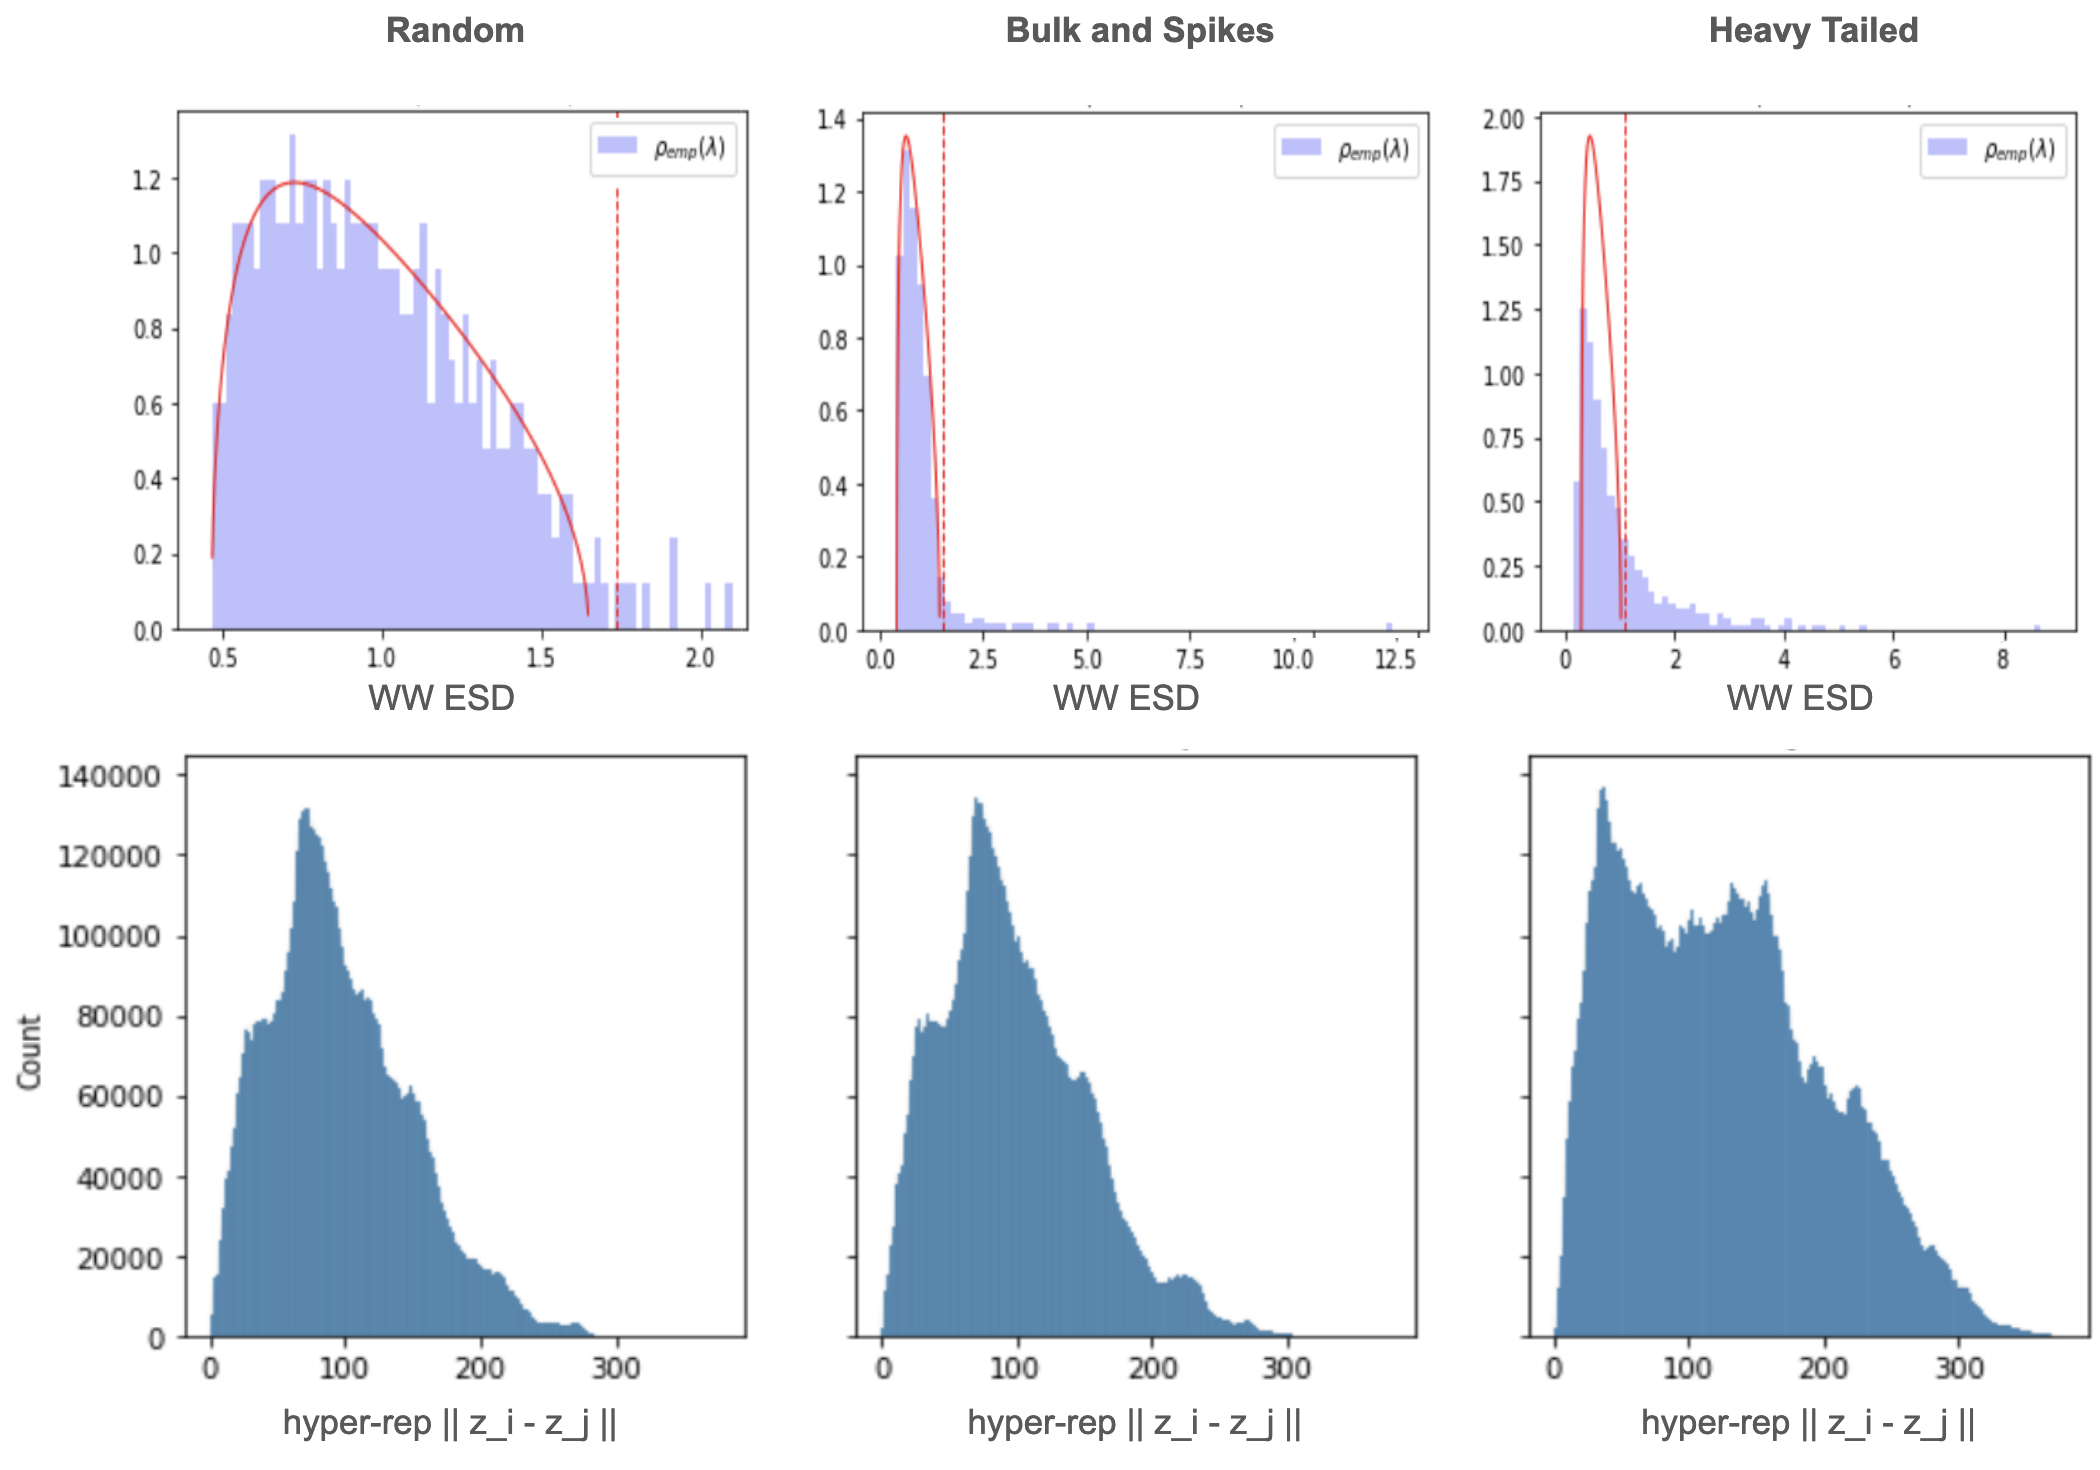
\includegraphics[trim=4mm 0mm 1.5mm 1.5mm, width=0.6\linewidth]{figures/ww_phases_comparison.png}
\captionof{figure}{Comparison between WeightWatcher features (top) and \ourmethod (bottom). \citet{martinTraditionalHeavyTailedSelf2019} identify different phases in the eigenvalue spectrum of trained weight matrices. We replicate the experiment setup and find ESDs similar to \textit{random} (top left), \textit{bulk and spikes} (top middle) and \textit{heavy-tailed} (top right). We compare these against pairwise distances of \ourmethod embeddings of the same layer. While the distributions have a different shape, it appears to become more heavy-tailed going from \textit{random} to \textit{heavy tailed}.
}
\vspace{-2mm}
\label{fig:ww_comparison_phases}    
\end{figure}
%%%%%%%%%%%%
Figures \ref{fig:ww_comparison_layers_vgg} and \ref{fig:ww_comparison_layers_resnets_2x2} compare \ourmethod with different WeightWatcher metrics on VGGs from pytorchcv \citep{semeryOsmrImgclsmob2024} and the ResNet-18 zoo from the modelzoo dataset \citep{schurholtModelZoosDataset2022}.
%%%%%%%%%%%%
\begin{figure}[h!]
\centering
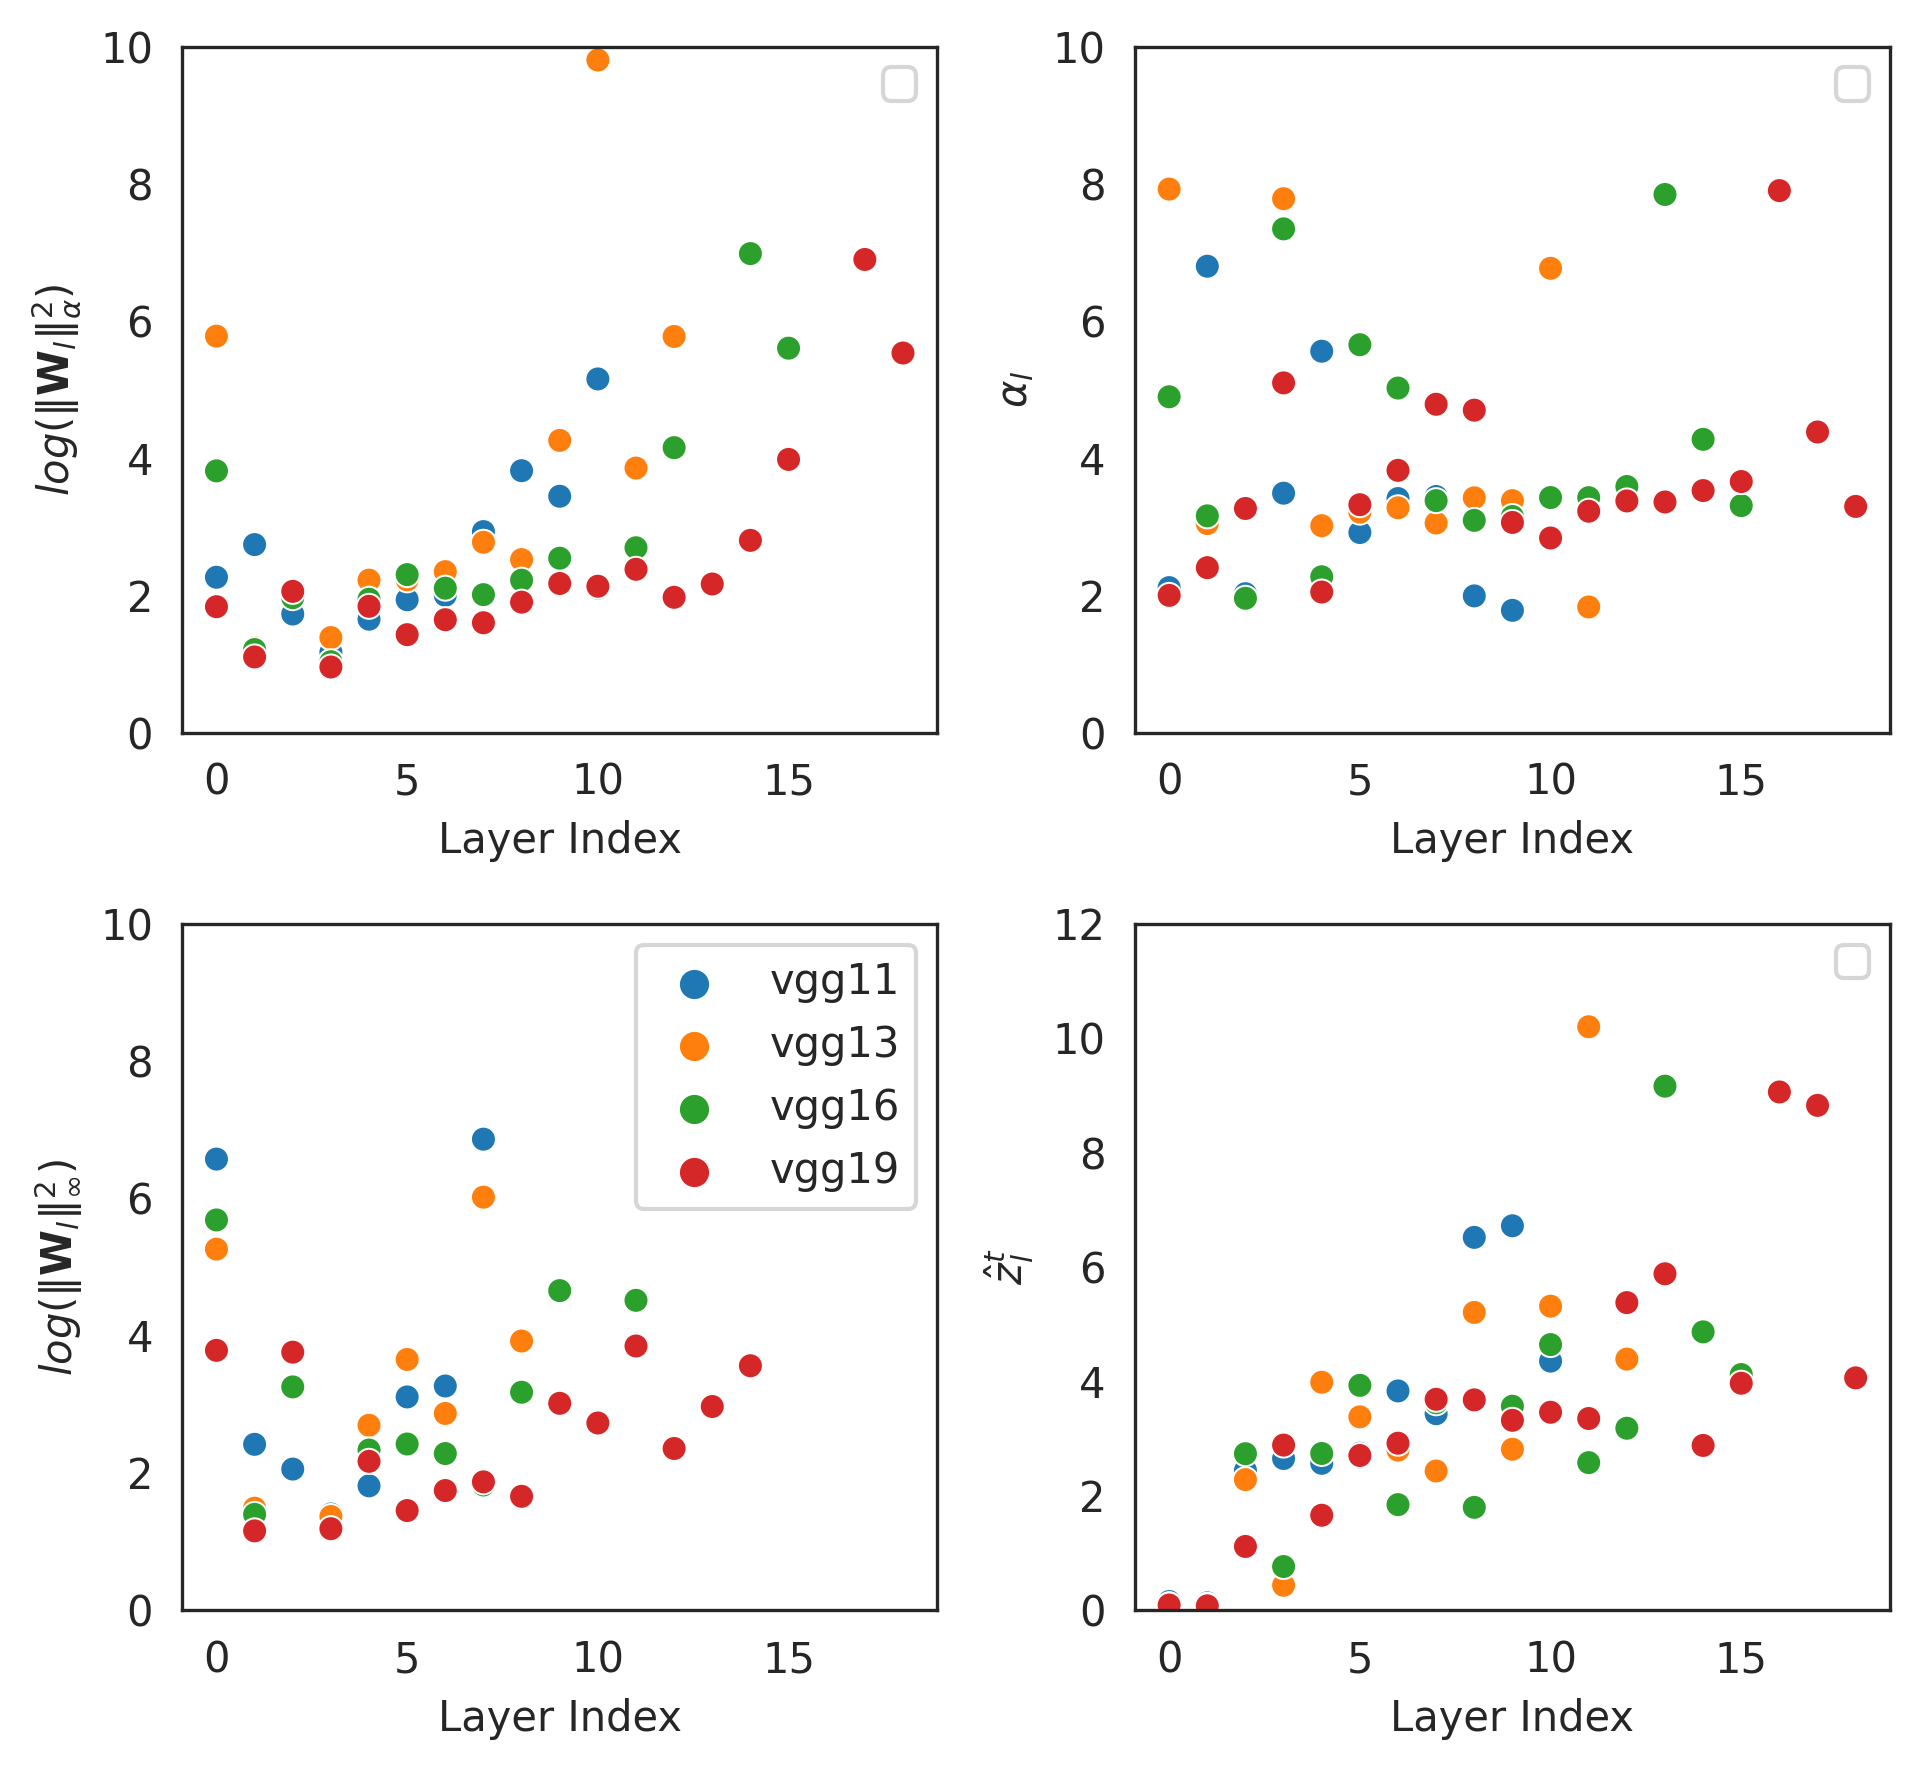
\includegraphics[trim=4mm 0mm 1.5mm 1.5mm, width=0.6\linewidth]{figures/ww_comparison_layers_2x2.png}
\captionof{figure}{Comparison between different WeightWatcher (WW) features (left) and \ourmethod (right). Features over layer index for VGGs from pytorchcv of different sizes. \ourmethod shows similar trends to WW, low values at early layers and a sharp increase at the end. }
\vspace{-2mm}
\label{fig:ww_comparison_layers_vgg}
\end{figure}
%%%%%%%%%%%%
%%%%%%%%%%%%
\begin{figure}[h!]
\centering
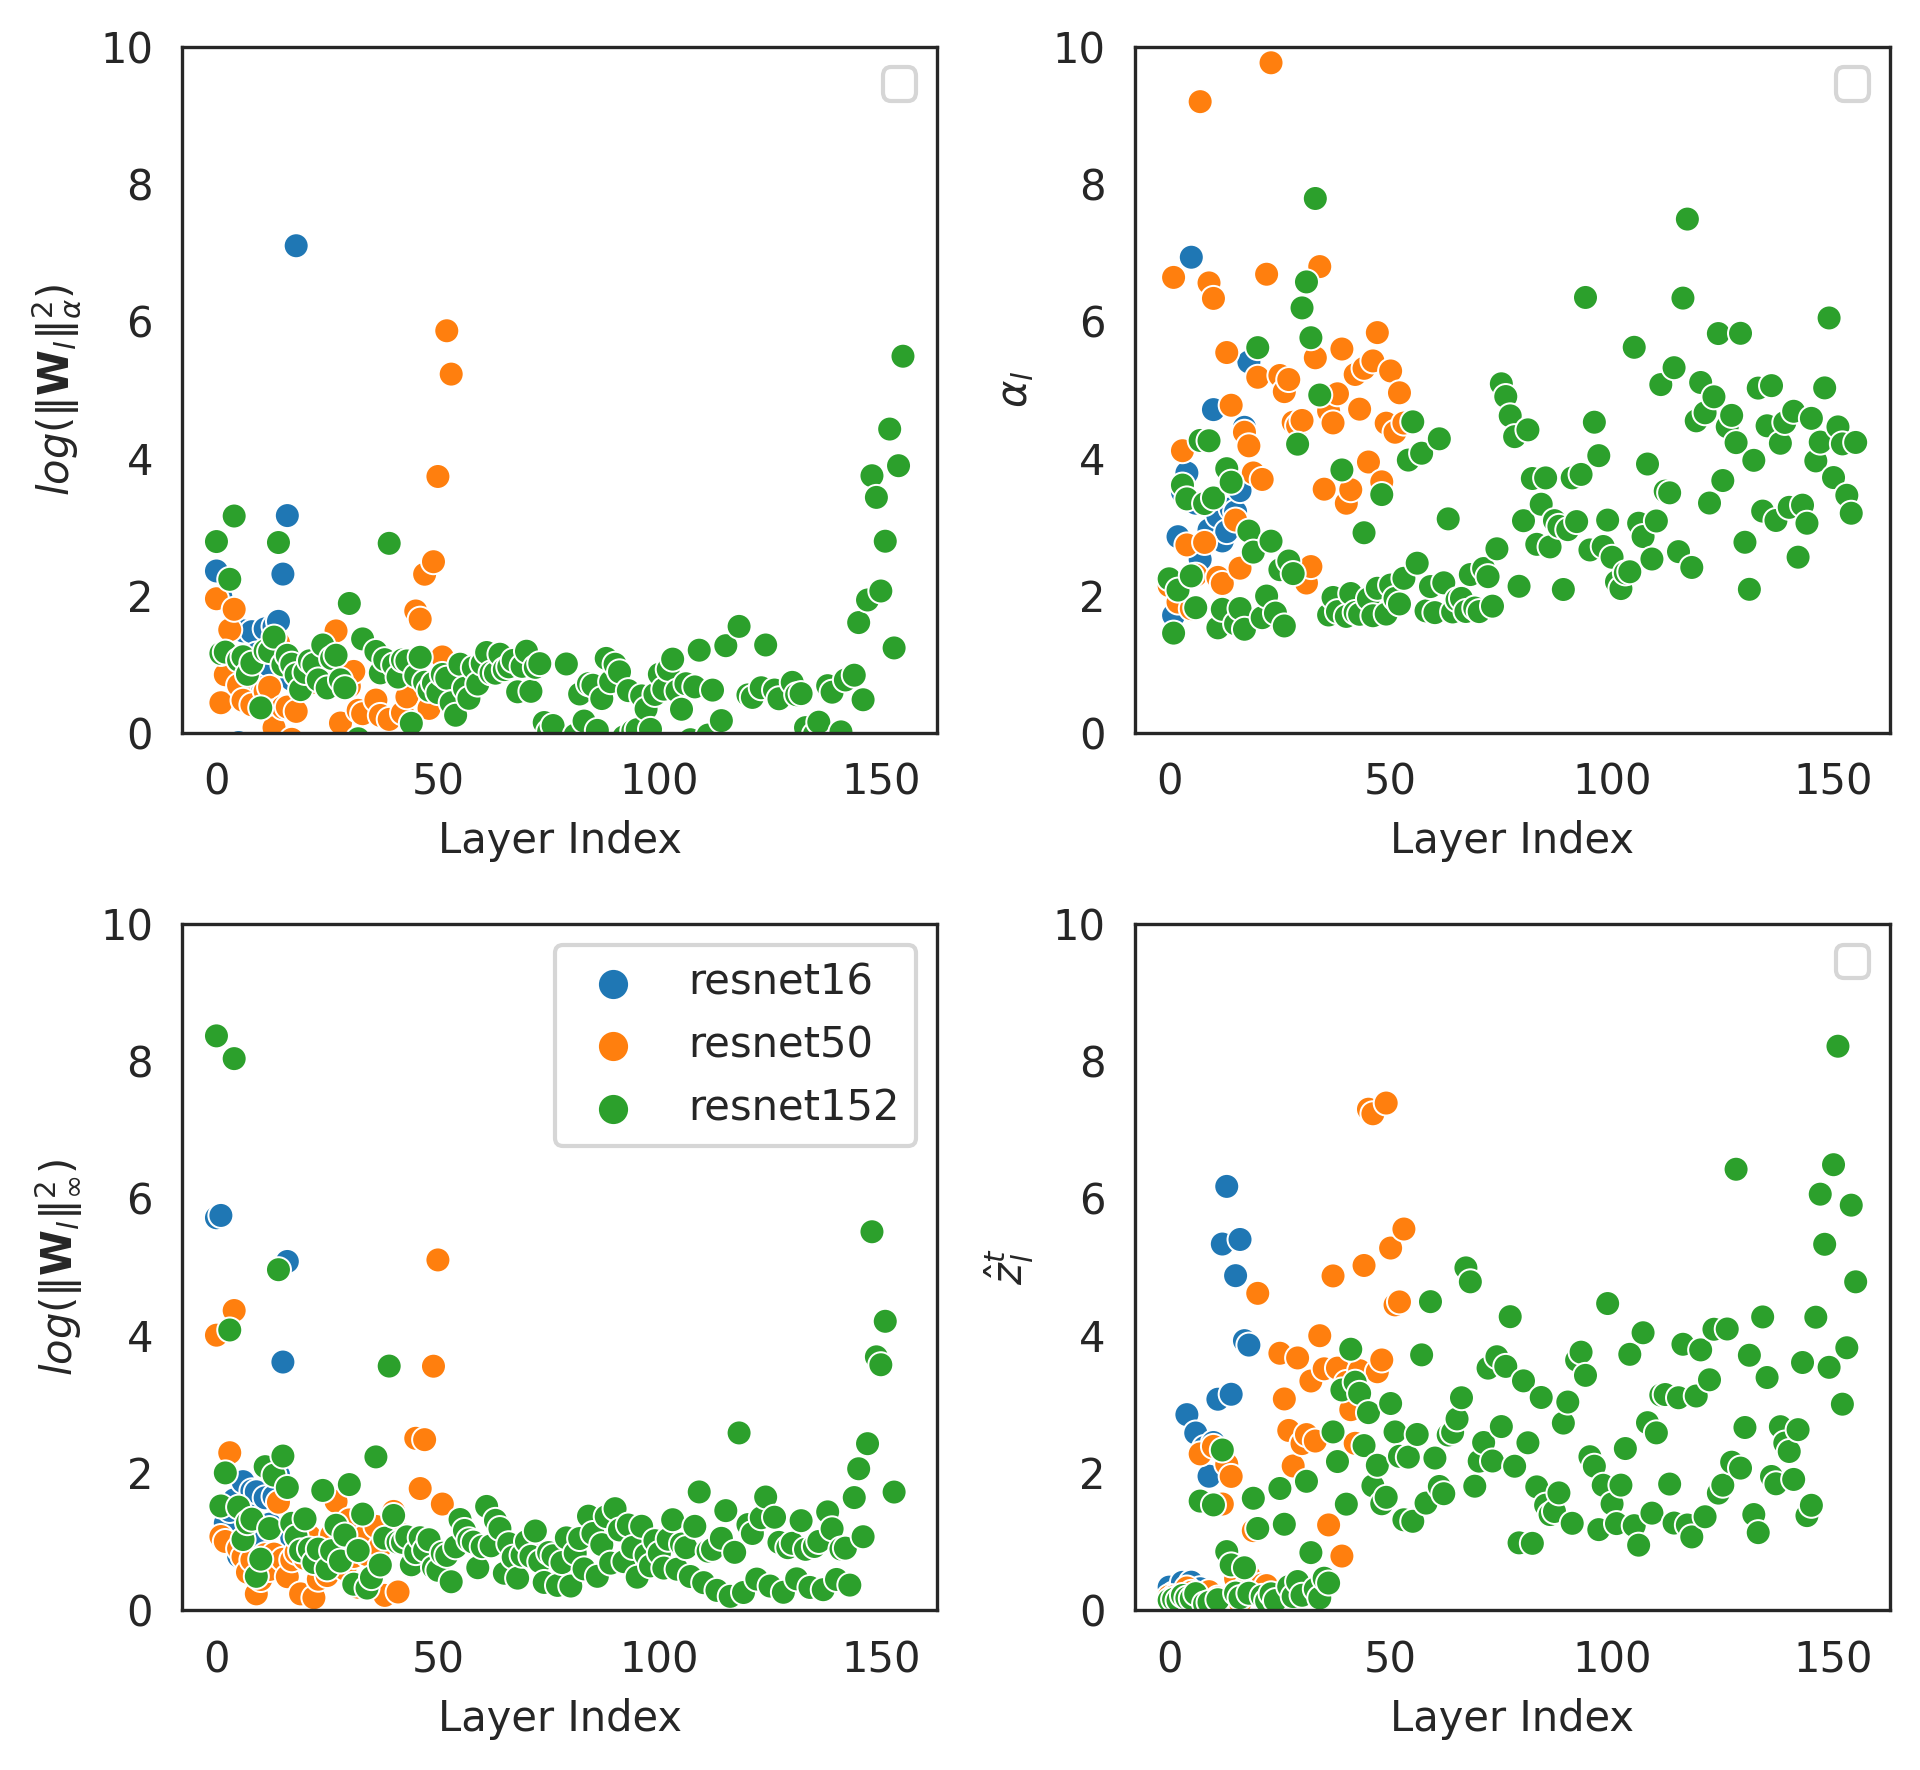
\includegraphics[trim=4mm 0mm 1.5mm 1.5mm, width=0.6\linewidth]{figures/ww_comparison_layers_2_2x2.png}
\captionof{figure}{Comparison between different WeightWatcher (WW) features (left) and \ourmethod (right). Features over layer index for Resnets from pytorchcv of different sizes. \ourmethod shows similar trends to WW, low values at early layers and a sharp increase at the end. }
\vspace{-2mm}
\label{fig:ww_comparison_layers_resnets_2x2}
\end{figure}
%%%%%%%%%%%%
%%%%%%%%%%%%
\begin{figure}[h!]
\centering
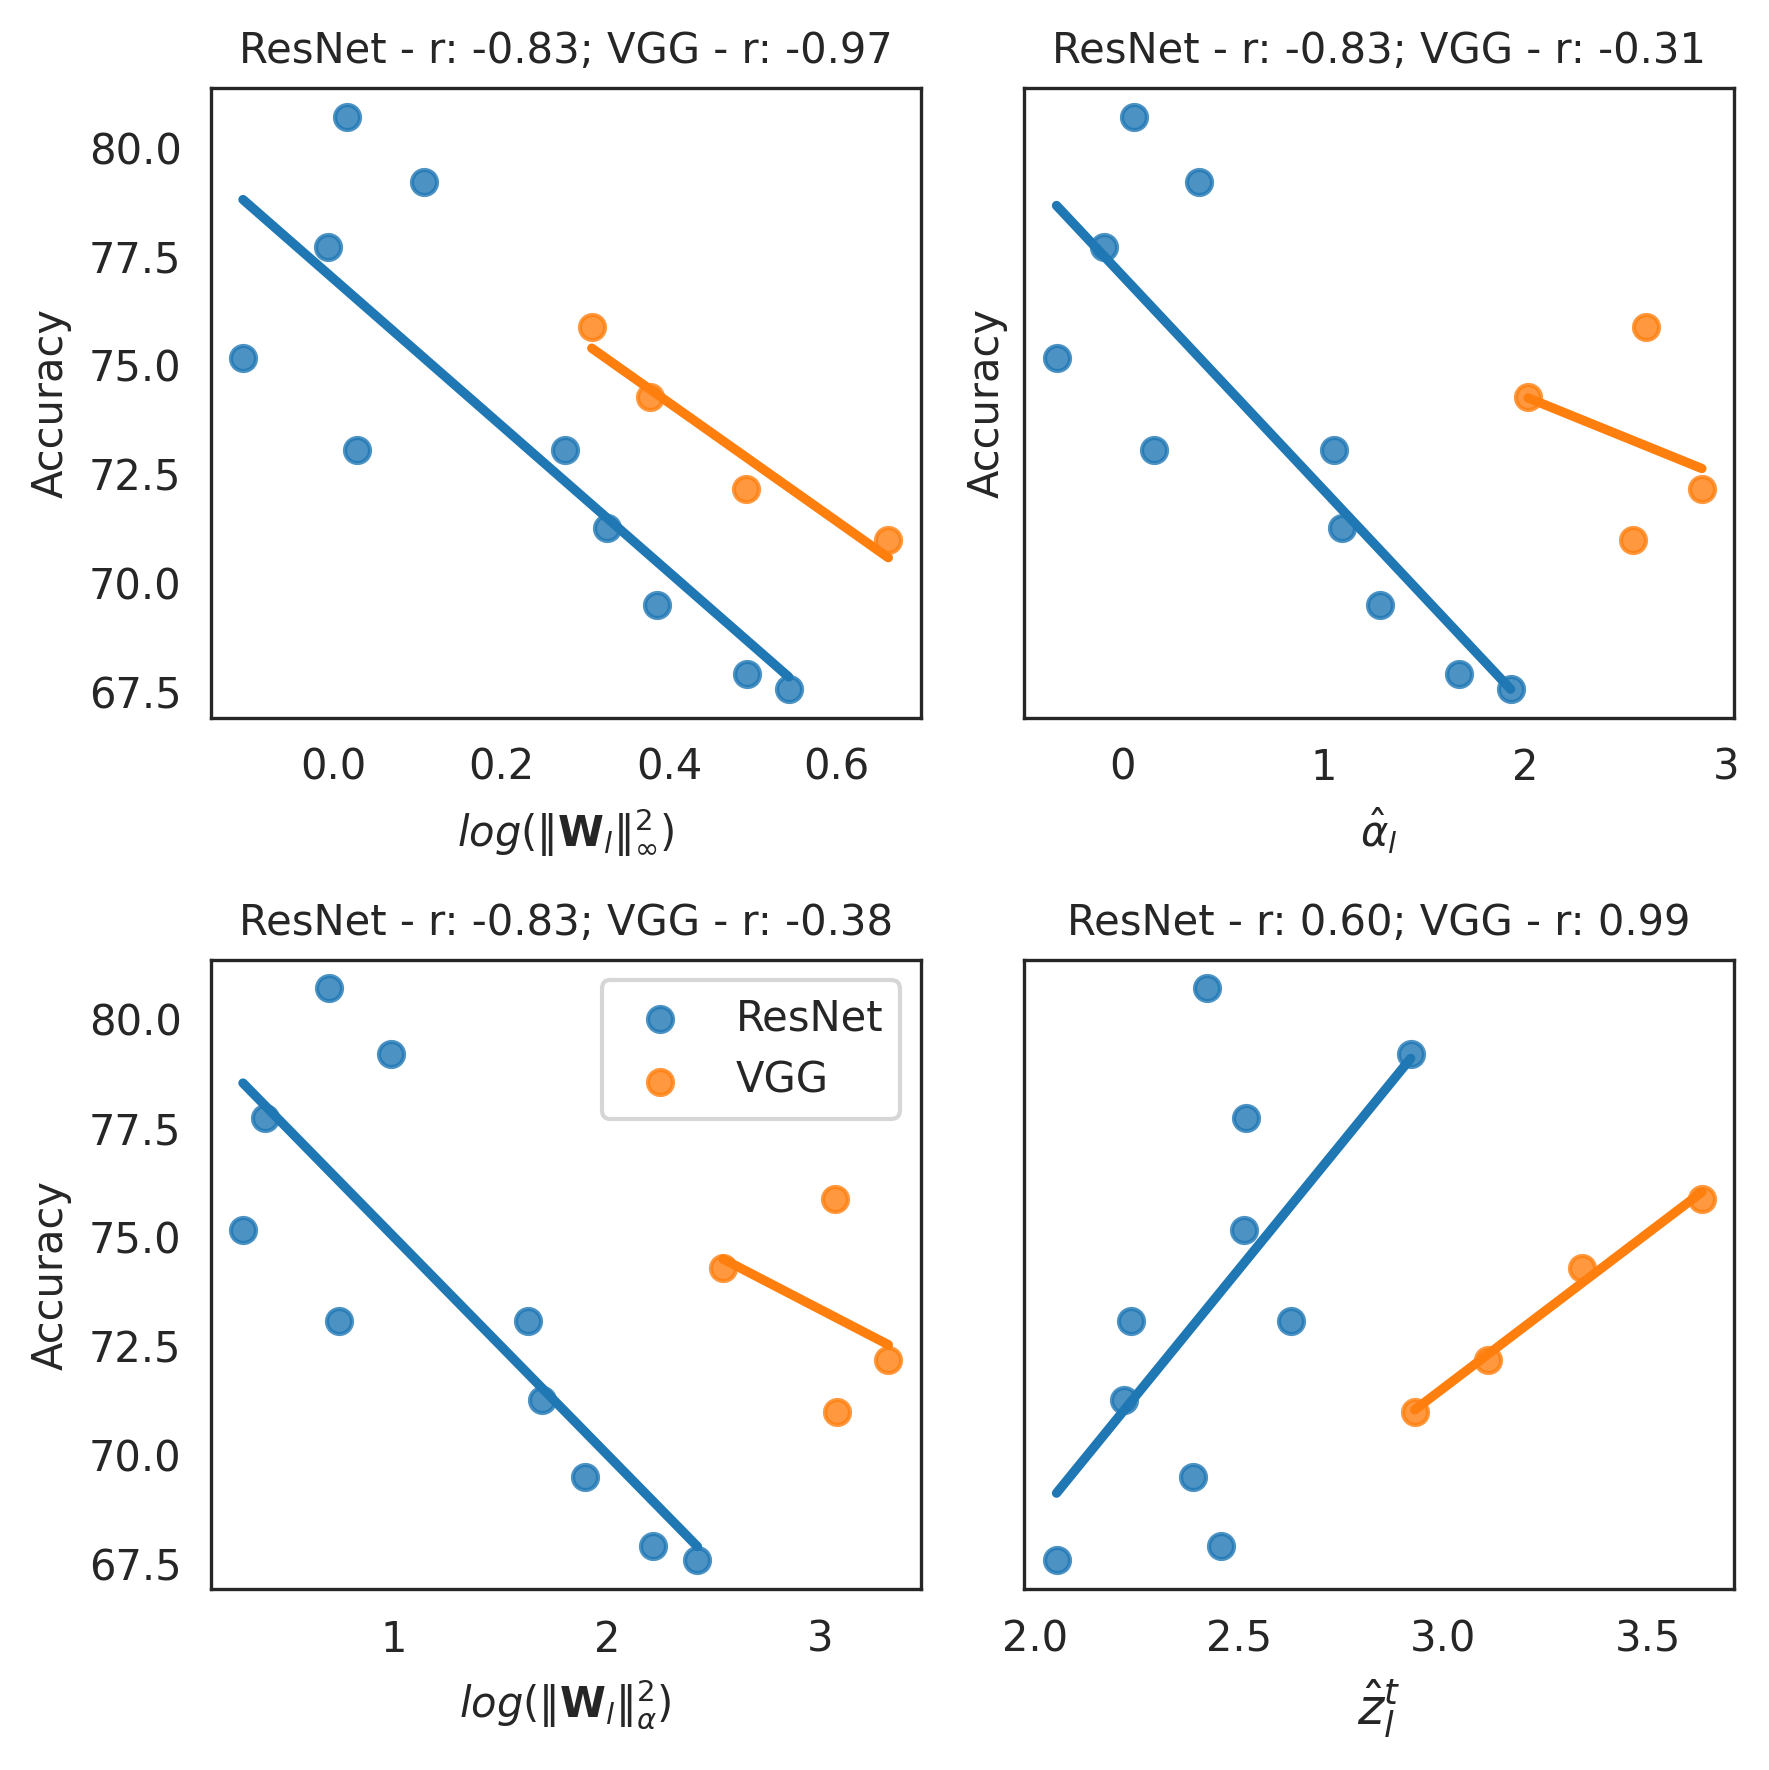
\includegraphics[trim=4mm 0mm 1.5mm 1.5mm, width=0.6\linewidth]{figures/ww_comparison_accuracy_2x2.png}
\captionof{figure}{Comparison between WeightWatcher features (left) and \ourmethod (right). Accuracy over model features for Resnets and VGGs from pytorchcv of different sizes. \ourmethod shows similar trends to WW, low values at early layers and a sharp increase at the end. }
\vspace{-2mm}
\label{fig:ww_comparison_accuracy_2x2}
\end{figure}
%%%%%%%%%%%%
%%%%%%%%%%%%
\begin{figure}[h!]
\centering
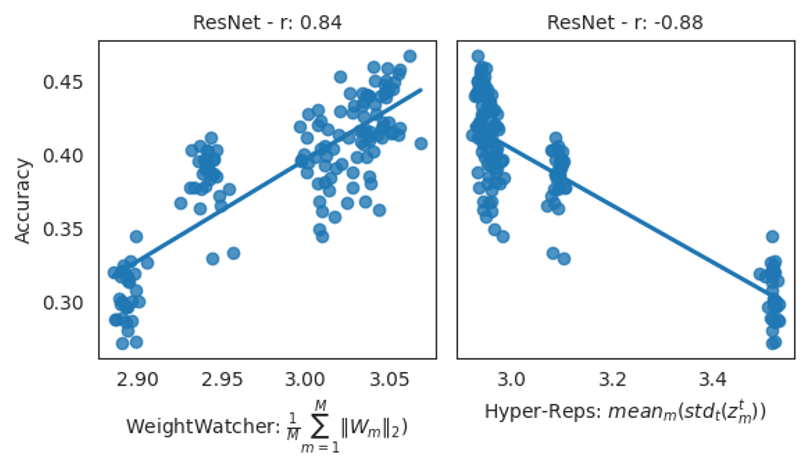
\includegraphics[trim=4mm 0mm 1.5mm 1.5mm, width=0.6\linewidth]{figures/ww_comparison_accuracy_2.png}
\captionof{figure}{Comparison between WeightWatcher features (left) and \ourmethod (right). Accuracy over model features for ResNets from the ResNet model zoo. Although \ourmethod is pretrained in a self-supervised fashion, it preserves the linear relation of a globally-aggregated embedding to model accuracy.}
\vspace{-2mm}
\label{fig:ww_comparison_accuracy_our_zoo}    
\end{figure}
%%%%%%%%%%%%


\section{Model Property Prediction - Additional Results}
In this section, we provide additional details for Section \ref{sec:property_prediction}. Table \ref{tab:discr_small_zoos_full} shows full results for populations of small CNNs. 
\begin{table}[h!]
\centering
\captionof{table}{
Property prediction on populations of small CNNs. 
}
\label{tab:discr_small_zoos_full}
\scriptsize
\setlength{\tabcolsep}{5pt}
\begin{tabularx}{0.8\linewidth}{lccccccccccccccc}
\toprule
      & \multicolumn{3}{c}{MNIST}                                                      &  & \multicolumn{3}{c}{SVHN}                                                       &  & \multicolumn{3}{c}{CIFAR-10 (CNN)}                                             &  & \multicolumn{3}{c}{STL}                                                        \\ 
      \cmidrule(r){2-4} \cmidrule(lr){6-8} \cmidrule(lr){10-12} \cmidrule(l){14-16} 
      & \multicolumn{1}{c}{W} & \multicolumn{1}{c}{$s(W)$} & \multicolumn{1}{c}{\ourmethod} &  & \multicolumn{1}{c}{W} & \multicolumn{1}{c}{$s(W)$} & \multicolumn{1}{c}{\ourmethod} &  & \multicolumn{1}{c}{W} & \multicolumn{1}{c}{$s(W)$} & \multicolumn{1}{c}{\ourmethod} &  & \multicolumn{1}{c}{W} & \multicolumn{1}{c}{$s(W)$} & \multicolumn{1}{c}{\ourmethod} \\ 
      \cmidrule(r){1-1} \cmidrule(r){2-4} \cmidrule(lr){6-8} \cmidrule(lr){10-12} \cmidrule(l){14-16} 
ACC   & 0.965                 & \textbf{0.987}           & 0.978                       &  & 0.910                 & 0.985                    & \textbf{0.991}              &  & -7.580                & \textbf{0.965}           & 0.885                       &  & -18.818               & \textbf{0.919}           & 0.305                       \\
Epoch & 0.953                 & \textbf{0.974}           & 0.958                       &  & 0.833                 & \textbf{0.953}           & 0.930                       &  & 0.636                 & \textbf{0.923}           & 0.771                       &  & -1.926                & \textbf{0.977}           & 0.344                       \\
Ggap  & 0.246                 & 0.393                    & \textbf{0.402}              &  & 0.479                 & 0.711                    & \textbf{0.760}              &  & 0.324                 & \textbf{0.909}           & 0.772                       &  & -0.617                & \textbf{0.858}           & 0.307                       \\ \bottomrule
\end{tabularx}
\end{table} 

\subsection{Comparison to Previous Work}
\label{app:discr_comparison_previous_work}
Here, we compare \ourmethod with previous work to disseminate the information contained in model embeddings.
The experiment setup in this paper is designed around the ResNets, and therefore it uses sparse epochs for computational efficiency. For consistency, we use the same setup for the CNN zoos as well. The exact numbers are therefore not directly comparable to \citet{schurholtSelfSupervisedRepresentationLearning2021}.   
To provide as much context as possible, we approach the comparison from two angles:
\begin{itemize}
    \item [(1)]\textbf{Direct comparison to the published results:} to contextualize, we use the (deterministic) results of weight statistics $s(W)$ to adjust for the differences in setup. We mark the results for $s(W)$ from \citet{schurholtSelfSupervisedRepresentationLearning2021} as $s(W)_{pp}$ and compare to their $E_{c+}D$ where possible.
    \item [(2)] \textbf{Approximation of the effect of global embeddings:} previous work used global model embeddings, which we approximate by using the full model embedding sequence. We therefore compare \ourmethod + aggregated tokens (as proposed in the submission) to \ourmethod + full model sequence (similar to \citet{schurholtSelfSupervisedRepresentationLearning2021}).
\end{itemize}

The results in the Tables below allow the following conclusions:
\begin{itemize}
    \item [(1)] \textbf{\ourmethod matches the performance of previous work:} The only data available for direct comparison is the MNIST zoo. Here, both in direct comparison and in relation to s(W) cross-relating our results with published numbers, \ourmethod matches published performance of $E_c+D$. On other zoos, $E_c+D$ had similar performance to $s(W)$. We likewise find \ourmethod embeddings to have similar performance to $s(W)$ in our experiments.
    \item [(2)] \textbf{\ourmethod + full sequence improves downstream task performance over the \ourmethod + aggregated sequence:} That indicates that \ourmethod + full sequence contains more information for model prediction. However, both \citet{schurholtSelfSupervisedRepresentationLearning2021} and \ourmethod with full sequence have the disadvantage that they do not scale. With growing models, the representation learner of \citet{schurholtSelfSupervisedRepresentationLearning2021} and the input to the linear probe of \ourmethod + full sequence grow accordingly. \ourmethod + aggregated sequence does lose some information on small models, but scales gracefully to large models and remains competitive.
\end{itemize}

%%%%%%%%%%%%%%%%%%%%%
\begin{table}[h!]
\small
\centering
\caption{Property Prediction comparison to previous work on the MNIST-CNN model zoo. We compare our linear probing results from weights $W$, layer-wise quintiles $s(W)$, embeddings from \ourmethod either aggregated into one embedding or using the full sequence to results previously published in \citet{schurholtSelfSupervisedRepresentationLearning2021}. We mark their results for $s(W)$ as $s(W)_{pp}$. Since the experimental setup is not the same, the numbers of $s(W)$ do not match.}
\setlength{\tabcolsep}{8pt}
\begin{tabularx}{0.75\linewidth}{ccccccc}
\toprule
      & \multicolumn{1}{c}{W} & \multicolumn{1}{c}{$s(W)$} & \multicolumn{1}{c}{\ourmethod aggregated} & \ourmethod full sequence & \multicolumn{1}{c}{$s(W)_{pp}$} & \multicolumn{1}{c}{$E_{c+}D$} \\
\cmidrule(r){1-1} \cmidrule(lr){2-2} \cmidrule(lr){3-3} \cmidrule(lr){4-4} \cmidrule(lr){5-5} \cmidrule(lr){6-6} \cmidrule(l){7-7}  
ACC   & 0.965                 & \textbf{0.987}           & 0.978                               & \textbf{0.987}     & 0.977                            & 0.973                              \\
Epoch & 0.953                 & 0.974                    & 0.958                               & \textbf{0.975}     & 0.987                            & 0.989                              \\
Ggap  & 0.246                 & 0.393                    & 0.402                               & \textbf{0.461}     & 0.662                            & 0.667     \\
\bottomrule
\end{tabularx}
\label{tab:discr_comparison_mnist}
\end{table}
%%%%%%%%%%%%%%%%%%%%%%%%%%%%%%%%%%%%%%%%%%%%%%%%%%%%%%%%%%%%%%%%%%%%%%%%%%%%%%%%%%%%%%%%%%%%%%%%%%%
%%%%%%%%%%%%%%%%%%%%%
\begin{table}[h!]
\small
\centering
\caption{Property Prediction comparison to previous work on the SVHN-CNN model zoo. We compare our linear probing results from weights $W$, layer-wise quintiles $s(W)$, to embeddings from \ourmethod either aggregated into one embedding or using the full sequence. For this zoo, previous results are not available.}
\setlength{\tabcolsep}{8pt}
\begin{tabularx}{0.75\linewidth}{ccccccc}
\toprule
      & \multicolumn{1}{c}{W} & \multicolumn{1}{c}{$s(W)$} & \multicolumn{1}{c}{\ourmethod aggregated} & \ourmethod full sequence & \multicolumn{1}{c}{$s(W)_{pp}$} & \multicolumn{1}{c}{$E_{c+}D$} \\
\cmidrule(r){1-1} \cmidrule(lr){2-2} \cmidrule(lr){3-3} \cmidrule(lr){4-4} \cmidrule(lr){5-5} \cmidrule(lr){6-6} \cmidrule(l){7-7}  
ACC   & 0.910                 & \textbf{0.985}           & 0.991                               & \textbf{0.993}     & \textit{n/a}         & \textit{n/a}         \\
Epoch & 0.833                 & \textbf{0.953}           & 0.930                               & \textbf{0.943}     & \textit{n/a}         & \textit{n/a}         \\
Ggap  & 0.479                 & 0.711                    & 0.760                               & \textbf{0.77}      & \textit{n/a}         & \textit{n/a}        \\
\bottomrule
\end{tabularx}
\label{tab:discr_comparison_svhn}
\end{table}
%%%%%%%%%%%%%%%%%%%%%%%%%%%%%%%%%%%%%%%%%%%%%%%%%%%%%%%%%%%%%%%%%%%%%%%%%%%%%%%%%%%%%%%%%%%%%%%%%%%

%%%%%%%%%%%%%%%%%%%%%
\begin{table}[h!]
\small
\centering
\caption{Property Prediction comparison to previous work on the CIFAR-CNN(m) model zoo. We compare our linear probing results from weights $W$, layer-wise quintiles $s(W)$, to embeddings from \ourmethod either aggregated into one embedding or using the full sequence. For this zoo, previous results are not available.}
\setlength{\tabcolsep}{8pt}
\begin{tabularx}{0.75\linewidth}{ccccccc}
\toprule
      & \multicolumn{1}{c}{W} & \multicolumn{1}{c}{$s(W)$} & \multicolumn{1}{c}{\ourmethod aggregated} & \ourmethod full sequence & \multicolumn{1}{c}{$s(W)_{pp}$} & \multicolumn{1}{c}{$E_{c+}D$} \\
\cmidrule(r){1-1} \cmidrule(lr){2-2} \cmidrule(lr){3-3} \cmidrule(lr){4-4} \cmidrule(lr){5-5} \cmidrule(lr){6-6} \cmidrule(l){7-7}  
ACC   & -7.580                & \textbf{0.965}           & 0.885                               & \textbf{0.947}     & \textit{n/a}         & \textit{n/a}         \\
Epoch & 0.636                 & \textbf{0.923}           & 0.771                               & \textbf{0.879}     & \textit{n/a}         & \textit{n/a}         \\
Ggap  & 0.324                 & \textbf{0.909}           & 0.772                               & \textbf{0.811}     & \textit{n/a}         & \textit{n/a}        \\
\bottomrule
\end{tabularx}
\label{tab:discr_comparison_cifar}
\end{table}
%%%%%%%%%%%%%%%%%%%%%%%%%%%%%%%%%%%%%%%%%%%%%%%%%%%%%%%%%%%%%%%%%%%%%%%%%%%%%%%%%%%%%%%%%%%%%%%%%%%




%%%%%%%%%%%%%%%%%%%%%%%%%%%%%%%%%%%%%%%%%%%%%%%%%%%%%%%%%%%%%%%%%%%%%%%%%%%%
\section{Model Generation - Additional Results}
This section contains additional results from model sampling experiments, extending Section \ref{sec:generating_models}. 
In Table \ref{tab:generative_cnn_zoos_transfer}, we show results on small CNNs transferring to a new task.
Similarly, Table \ref{tab:generative_resnets_zoos_transfer} shows results on ResNet-18 models for task transfers.
Lastly, Tables \ref{tab:generative_resnets_zoos_fewshot_resnet34}, \ref{tab:generative_resnets_zoos_fewshot_ti_resnet34} and \ref{tab:generative_resnets_zoos_fewshot_resnet34_one_prompt_example} contain additional results for transferring from ResNet-18 CIFAR-100 to ResNet34 and/or Tiny-Imagenet. 
%%%%%%%%%%%%%%%%%%%%%
\begin{table}[h!]
\small
\centering
\caption{Model generation on CNN model populations transfer learned on a new task. We compare sampled models at different epochs with models trained from scratch and models fine-tuned from the anchor samples.}
\setlength{\tabcolsep}{8pt}
\begin{tabularx}{0.75\linewidth}{ccccccc}
\toprule
  Method              & \multicolumn{3}{c}{SVHN to MNIST}                            & \multicolumn{3}{c}{CIFAR-10 to STL-10}                       \\
\cmidrule(r){1-1} \cmidrule(lr){2-4} \cmidrule(lr){5-7}
          & Epoch 0            & Epoch 1            & Epoch 25           & Epoch 0            & Epoch 1            & Epoch 25           \\
\cmidrule(r){1-1} \cmidrule(lr){2-2} \cmidrule(lr){3-3} \cmidrule(lr){4-4} \cmidrule(lr){5-5} \cmidrule(lr){6-6} \cmidrule(l){7-7}  
tr.fr.scratch   & $\sim$10 /\%       & 20.6+-1.6          & 83.3+-2.6          & $\sim$10 /\%       & 21.3+-1.6          & 44.0+-1.0          \\
pretrained      & 29.1+-7.2          & 84.1+-2.6          & 94.2+-0.7          & 16.2+-2.3          & 24.8+-0.8          & 49.0+-0.9          \\
$S_{KDE30}$      &  31.8+-5.6          &  86.9+-1.4          &  95.5+-0.4          & n/a          & n/a          & n/a          \\
\cmidrule(r){1-1} \cmidrule(lr){2-2} \cmidrule(lr){3-3} \cmidrule(lr){4-4} \cmidrule(lr){5-5} \cmidrule(lr){6-6} \cmidrule(l){7-7}  
\ourmethod$_{KDE30}$ & \textbf{40.2+-4.8} & 86.7+-1.6          & 94.8+-0.4          & 15.5+-2.3          & 24.9+-1.6          & 49.2+-0.5          \\
\ourmethod$_{SUB}$.  & 37.9+-2.8          & \textbf{88.2+-0.5} & \textbf{95.6+-0.3} & \textbf{17.4+-1.4} & \textbf{25.6+-1.7} & \textbf{49.8+-0.6} \\
\bottomrule
\end{tabularx}
\label{tab:generative_cnn_zoos_transfer}
\end{table}
%%%%%%%%%%%%%%%%%%%%%%%%%%%%%%%%%%%%%%%%%%%%%%%%%%%%%%%%%%%%%%%%%%%%%%%%%%%%%%%%%%%%%%%%%%%%%%%%%%%



%%%%%%%%%%%%%%%%%%%%%%%%%%%%%%%%%%%%%%%%%%%%%%%%%%%%%%%%%%%%%%%%%%%%%%%%%%%%%%%%%%%%%%%%%%%%%%%%%%
\begin{table}[]
\scriptsize
\centering
\caption{Model generation on ResNet-18 model populations transferred to a new task. We compare sampled models at different transfer learning epochs with models trained from scratch and models fine-tuned from the same anchor samples.}
\setlength{\tabcolsep}{6pt}
\begin{tabularx}{0.75\linewidth}{clccc}
\toprule
Epoch                  & \multicolumn{1}{c}{Method} & CIFAR-10 to CIFAR-100 & CIFAR-100 to Tiny-Imagenet & Tiny-Imagenet to CIFAR-100 \\
\cmidrule(r){1-1} \cmidrule(lr){2-2} \cmidrule(lr){3-3} \cmidrule(lr){4-4} \cmidrule(l){5-5} 
\multirow{5}{*}{0}     & tr. fr. scratch                  & $\sim$1 /\%                      & $\sim$0.5 /\%                        & $\sim$1 /\%                           \\
                       & Finetuned                  & 1.0+-0.3                     & 0.5+-0.0                             & 1.1+-0.2                              \\
                       & \ourmethod$_{KDE30}$                    & 1.0+-0.3                         & 0.5+-0.1                             & 1.0+-0.2                              \\
                       & \ourmethod$_{SUB}$                   & 1.0+-0.3                         & 0.6+-0.0                             & 1.1+-0.2                              \\
                       & \ourmethod$_{BOOT}$                  & 1.1+-0.2                         & 0.5+-0.0                             & 0.9+-0.2                              \\
\cmidrule(r){1-1} \cmidrule(lr){2-2} \cmidrule(lr){3-3} \cmidrule(lr){4-4} \cmidrule(l){5-5} 
\multirow{5}{*}{1}     & tr. fr. scratch                  & 17.5+-0.7                        & 13.8+-0.8                            & 17.5+-0.7                             \\
                       & Finetuned                  & 27.5+-1.3                     & 25.7+-0.5                            & 51.7+-0.5                             \\
                       & \ourmethod$_{KDE30}$                    & 26.8+-1.4                        & 21.5+-0.9                            & 40.2+-1.0                             \\
                       & \ourmethod$_{SUB}$                   & 26.4+-1.9                        & 21.5+-1.0                            & 40.63+-1.3                            \\
                       & \ourmethod$_{BOOT}$                  & 25.7\_01.9                       & 21.7+-1.0                            & 40.9+-0.8                             \\
\cmidrule(r){1-1} \cmidrule(lr){2-2} \cmidrule(lr){3-3} \cmidrule(lr){4-4} \cmidrule(l){5-5} 
\multirow{5}{*}{5}     & tr. fr. scratch                  & 36.5+-2.0                        & 31.1+-1.6                            & 36.5+-2.0                             \\
                       & Finetuned                  &          45.7+-1.0                        & 36.3+-2.5                            & 52.6+-1.3                             \\
                       & \ourmethod$_{KDE30}$                    & 44.5+-2.0                        & 36.3+-1.2                            & 47.2+-3.3                             \\
                       & \ourmethod$_{SUB}$                   & 45.6+-1.2                        & 35.8+-1.4                            & 49.8+-2.3                             \\
                       & \ourmethod$_{BOOT}$                  & 43.3+-2.4                        & \textbf{37.3+2.0}                    & 50.2+-3.4                             \\
\cmidrule(r){1-1} \cmidrule(lr){2-2} \cmidrule(lr){3-3} \cmidrule(lr){4-4} \cmidrule(l){5-5} 
\multirow{5}{*}{15}    & tr. fr. scratch                  & 53.3+-2.0                        & 38.5+-1.9                            & 53.3+-2.0                             \\
                       & Finetuned                  & 71.9+-0.1                     & 63.4+-0.2                            & \textbf{73.9+-0.3}                    \\
                       & \ourmethod$_{KDE30}$                    & 71.8+-0.3                        & \textbf{63.6+-0.2}                   & 73.4+-0.2                             \\
                       & \ourmethod$_{SUB}$                   & 72.0+-0.2                        & \textbf{63.6+-0.3}                   & 73.5+-0.2                             \\
                       & \ourmethod$_{BOOT}$                  & 71.9+-0.3                        & 63.4+-0.1                            & 73.7+-0.3                             \\
\cmidrule(r){1-1} \cmidrule(lr){2-2} \cmidrule(lr){3-3} \cmidrule(lr){4-4} \cmidrule(l){5-5} 
25 & tr. fr. scratch                  & 56.5+-2.0                        & 43.3+-1.9                            & 56.5+-2.0                             \\
50 & tr. fr. scratch                  & 70.7+-0.4                        & 57.3+-0.6                            & 70.7+-0.4                             \\
60 & tr. fr. scratch                  & 74.2+-0.3                        & 63.9+-0.5                            & 74.2+-0.3                         \\
\bottomrule
\end{tabularx}
\label{tab:generative_resnets_zoos_transfer}
\end{table}





\begin{table}[h]
\vspace{-4mm}
\centering
\captionof{table}{
Few-shot model generation for a new task: Sampling ResNet-34 models for CIFAR-100. \ourmethod was pretrained on CIFAR-100 ResNet-18s, 5 samples are drawn using subsampling. To get prompt examples, we train 3 ResNet-34 models on CIFAR-100 for 2 epochs to a mean accuracy of 26 \%. }
\label{tab:generative_resnets_zoos_fewshot_resnet34}
\small
\setlength{\tabcolsep}{7pt}
\begin{center}
\begin{tabularx}{0.4\linewidth}{clcc}
\toprule
\multicolumn{4}{c}{CIFAR100   ResNet-18 to ResNet-34}                 \\
\midrule
  Ep.   & \multicolumn{1}{c}{Method}  & 5 Epochs           & 15 Epochs          \\
\cmidrule(r){1-1}  \cmidrule(l){2-2} \cmidrule(l){3-4} 
0  & tr. fr. Scratch           & 1.0$\pm$0.1           & 1.0$\pm$0.1           \\
         & \ourmethod & \textbf{1.6$\pm$0.3}  & \textbf{1.6$\pm$0.3}  \\
\cmidrule(r){1-1}  \cmidrule(l){2-2} \cmidrule(l){3-4} 
 1  & tr. fr. Scratch           & 12.4$\pm$1.0          & 12.9$\pm$0.8          \\
         & \ourmethod & \textbf{16.8$\pm$0.7} & \textbf{23.1$\pm$0.3} \\
\cmidrule(r){1-1}  \cmidrule(l){2-2} \cmidrule(l){3-4} 
5  & tr. fr. Scratch           & 49.5$\pm$0.6          & 36.2$\pm$1.7          \\
         & \ourmethod & \textbf{51.9$\pm$0.6} & \textbf{37.8$\pm$1.4} \\
\cmidrule(r){1-1}  \cmidrule(l){2-2} \cmidrule(l){3-4} 
15 & tr. fr. scratch      &      & 68.8$\pm$0.4          \\
         & \ourmethod &                    & \textbf{69.3$\pm$0.3} \\
\cmidrule(r){1-1}  \cmidrule(l){2-2} \cmidrule(l){3-4} 
 & \ourmethod Ens.                & 53.5               & 71.3         \\
\bottomrule
\end{tabularx}
\end{center}
\vspace{-4mm}
\end{table} 
\begin{table}[h]
\vspace{-4mm}
\small
\captionof{table}{
Few-shot model generation for a new task and architecture: \ourmethod trained on CIFAR-100 ResNet-18s used to generate ResNet-34s for Tiny-Imagenet. 5 samples are drawn using subsampling. To get prompt examples, we train 3 ResNet-34 models on Tiny-Imagenet for 2 epochs to a mean accuracy of 28.5 \%. 
}
\label{tab:generative_resnets_zoos_fewshot_ti_resnet34}
\centering
\begin{center}
\setlength{\tabcolsep}{7pt}
\begin{tabularx}{0.45\linewidth}{clcc}
\multicolumn{4}{c}{ResNet-18   CIFAR100 to ResNet-34 Tiny-Imagenet}                           \\
\cmidrule(r){1-1}  \cmidrule(l){2-2} \cmidrule(l){3-4} 
Ep.               & Method                    & 5 epochs           & 15 epochs          \\
\cmidrule(r){1-1}  \cmidrule(l){2-2} \cmidrule(l){3-4} 
\multirow{2}{*}{0}  & tr. fr. Scratch           & 0.5$\pm$0.0           & 0.5$\pm$0.0           \\
                    & \ourmethod & 0.5$\pm$0.1           & 0.6$\pm$0.2           \\
\cmidrule(r){1-1}  \cmidrule(l){2-2} \cmidrule(l){3-4} 
\multirow{2}{*}{1}  & tr. fr. Scratch           & 10.5$\pm$1.4          & 11.9$\pm$1.9          \\
                    & \ourmethod & \textbf{13.3$\pm$0.5} & \textbf{18.5$\pm$0.7} \\
\cmidrule(r){1-1}  \cmidrule(l){2-2} \cmidrule(l){3-4} 
\multirow{2}{*}{5}  & tr. fr. Scratch           & 47.2$\pm$0.7          & 31.1$\pm$1.7          \\
                    & \ourmethod & \textbf{50.6$\pm$0.3} & \textbf{31.6$\pm$0.6} \\
\cmidrule(r){1-1}  \cmidrule(l){2-2} \cmidrule(l){3-4} 
\multirow{2}{*}{15} & \multicolumn{2}{l}{tr. fr. Scratch}            & 61.9$\pm$0.3          \\
                    & \ourmethod &                    & \textbf{62.7$\pm$0.3} \\
\cmidrule(r){1-1}  \cmidrule(l){2-2} \cmidrule(l){3-4} 
            & \ourmethod Ens.                           & 52                 & 65.1              
\\
\bottomrule
\end{tabularx}
\end{center}
\vspace{-4mm}
% \end{wraptable} 
\end{table}

\subsection{Diversity of sampled models}
\label{sec:sampling_diversity}
An interesting question is whether sampling \ourmethod generates versions of the same model. To test that,  we evaluate the diversity of samples generated with only a few few-shot examples by combining the models to ensembles. 
The improvements of the ensembles over the individual models demonstrate their diversity.
This indicates that given very few, early-stage prompt examples, sampling hyper-representations improves learning speed and performance in otherwise equal settings. 
Additionally, we conducted experiments with varying numbers of prompt examples, revealing that increasing the number of prompt examples enhances both performance and diversity. 
Nonetheless, even a single prompt example trained for just 2 epochs contains sufficient information to generate model samples that surpass those derived from random initialization; see Table \ref{tab:generative_resnets_zoos_fewshot_resnet34_one_prompt_example}.

\begin{table}[h]
\centering
\captionof{table}{
Sampling ResNet-34 models for CIFAR-100. \ourmethod was pretrained on CIFAR-100 ResNet-18s, 5 samples are drawn using subsampling. To get prompt examples, we train a single ResNet-34 model on CIFAR-100 for 2 epochs to an accuracy of 26 \%. 
}
\label{tab:generative_resnets_zoos_fewshot_resnet34_one_prompt_example}
\small
\begin{center}
\setlength{\tabcolsep}{7pt}
\begin{tabularx}{0.5\linewidth}{clcc}
\toprule
\multicolumn{4}{c}{CIFAR100   ResNet-18 to ResNet-34}                 \\
\cmidrule(r){1-1}  \cmidrule(l){2-2} \cmidrule(l){3-4} 
  Epoch   & \multicolumn{1}{c}{Method}  & 5 Epochs           & 15 Epochs          \\
\cmidrule(r){1-1}  \cmidrule(l){2-2} \cmidrule(l){3-4} 
0  & tr. fr. Scratch            & 1.0+-0.1           & 1.0+-0.1           \\
         & \ourmethod           & \textbf{1.5+-0.2}  & \textbf{1.6+-0.1}  \\
\cmidrule(r){1-1}  \cmidrule(l){2-2} \cmidrule(l){3-4} 
 1  & tr. fr. Scratch           & 12.4+-1.0          & 12.9+-0.8          \\
         & \ourmethod           & \textbf{16.9+-0.7} & \textbf{19.4+-0.2} \\
\cmidrule(r){1-1}  \cmidrule(l){2-2} \cmidrule(l){3-4} 
5  & tr. fr. Scratch            & 49.5+-0.6          & 36.2+-1.7          \\
         & \ourmethod           & \textbf{51.5+-0.3} & \textbf{38.6+-1.6} \\
\cmidrule(r){1-1}  \cmidrule(l){2-2} \cmidrule(l){3-4} 
15 & tr. fr. scratch            &      &             68.8+-0.4          \\
         & \ourmethod &                              & \textbf{69.1+-0.1} \\
\cmidrule(r){1-1}  \cmidrule(l){2-2} \cmidrule(l){3-4} 
Ensemble & \ourmethod                & 51.8          & 70.2              
\\
\bottomrule
\end{tabularx}
\end{center}
\end{table} 
